\begin{figure}[H]
\centering
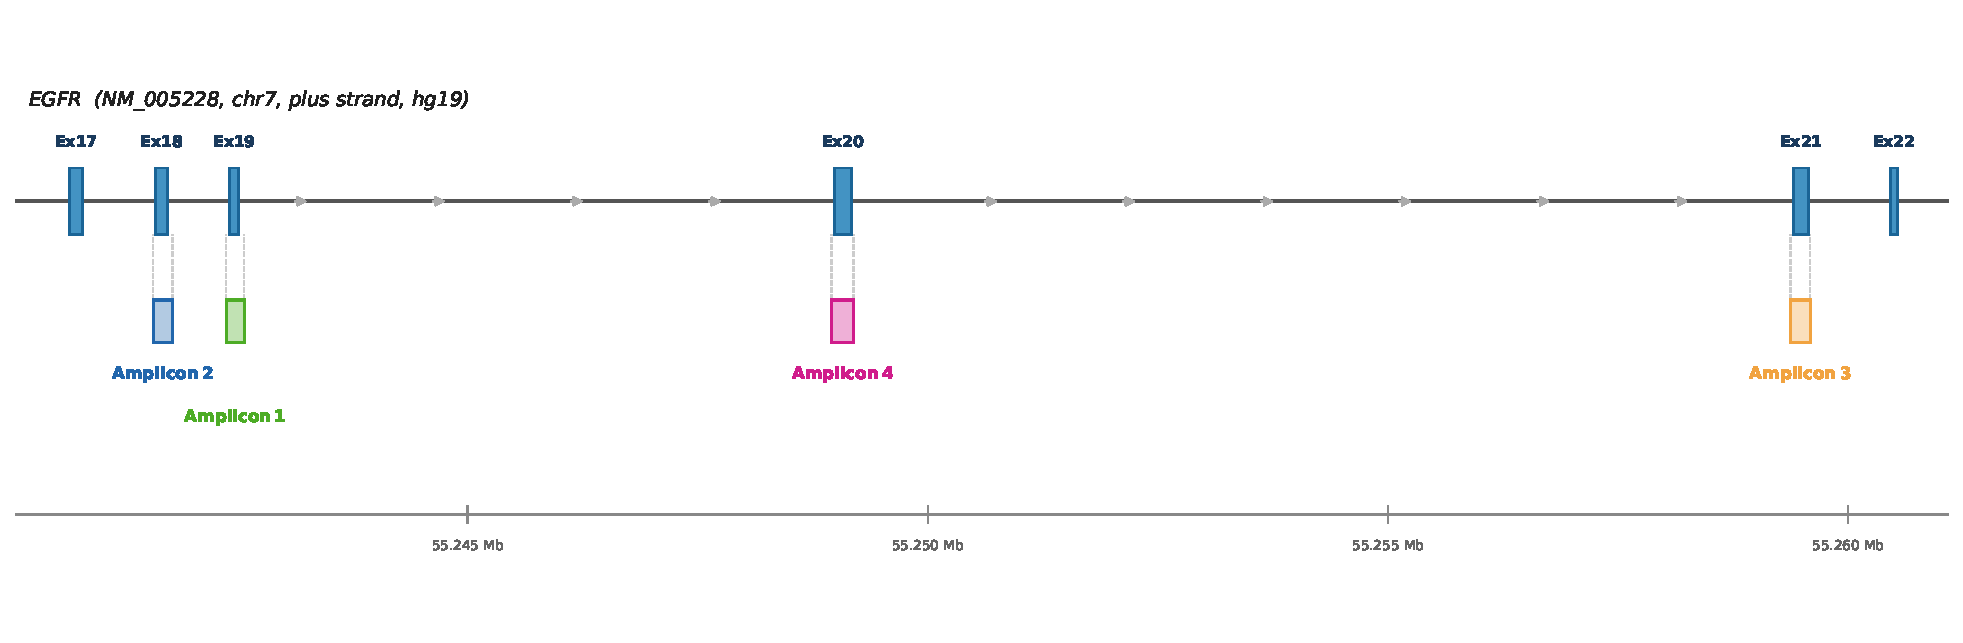
\includegraphics[width=\textwidth]{figures/egfr_exon_figure.pdf}
\caption{Exon structure of EGFR (NM\_005228, hg19, chr7 plus strand) in the region
targeted by the amplicon panel. Blue boxes indicate exons; exon numbers follow the
canonical transcript order (5$'$ to 3$'$, left to right). The four amplicons (coloured
bars) were localised by BLAST primer alignment (Table~\ref{tab:blast-primers-relaxed}).
Each amplicon spans exactly one exon: Amplicon~2 covers exon~18 (G719 mutation site),
Amplicon~1 covers exon~19 (the most common site of in-frame deletions in
NSCLC~\cite{lynch2004}), Amplicon~4 covers exon~20 (insertion hotspot), and
Amplicon~3 covers exon~21 (L858R substitution site~\cite{lynch2004}).
Together the four amplicons span the full kinase-domain mutational hotspot (exons~18--21).
Genomic coordinates are hg19 (GRCh37).}
\label{fig:egfr-exon}
\end{figure}
